%% Example of a LaTeX source file for a COLING-2012 submission
%% last updated: July 10, 2012
%% Optional instructions for authors within the tex file are provided as comments and start with 'for authors:...'
\documentclass[10pt,a5paper,twoside]{article}
\usepackage{coling2012}
\usepackage[vlined,algoruled,titlenumbered,noend]{algorithm2e}
\usepackage{amsmath,amsfonts,amssymb,amsthm}
\usepackage{array}
\usepackage{amsmath,amssymb}
\usepackage{epsfig,subfigure}
\usepackage{pgfplots}
\newcommand{\fix}{\marginpar{FIX}}
\newcommand{\new}{\marginpar{NEW}}
\newcommand{\ind}[1]{\mathbb{I}[#1]}
\newcommand{\inde}{\mathbb{I}}

\newcommand{\var}{v}
\newcommand{\eq}{\leftarrow}

\newcommand{\LB}{\mathit{LB}}
\newcommand{\UB}{\mathit{UB}}

\newcommand{\B}{\mathbb{B}}
\newcommand{\E}{\mathbb{E}}
\newcommand{\I}{\mathbb{I}}
\newcommand{\R}{\mathbb{R}}
\renewcommand{\vec}[1]{\mathbf{#1}}
%\title{United We Stand: Tweet Pooling for a better LDA}
\title{Improving LDA Topic Models for Microblogs\\ via Automatic Tweet Labeling and Pooling}
%for authors: in case of more than four author names ref. to commented line below 
%\author{$Annie~SMITH^{1, 2}~~~LI~Xiao Dong^{1, 3}$\\$~~~Third~Author^{1, 2}~~~Fourth~Author^{1, 3}~~~ Fifth~Author^{2, 3}$\\
\author{$Author1^{1}~~~Author2^{2}$\\
{\small  	(1) INSTITUTE\_1, address 1\\ 
 		(2) INSTITUTE\_2, address 2\\
  \texttt{mail-id, mail-id} \\ 
}}

\begin{document}
\maketitle

\abstractEn{ Twitter : the world of 140 characters poses serious
  challenges to the efficacy of topic models on short, messy text.
  While topic models such as Latent Dirichlet Allocation (LDA) have a
  long history of successful application to news articles and academic
  abstracts, they are often less coherent when applied to microblog
  content like Twitter.  In this paper, we investigate methods to
  improve topics learned from Twitter content \emph{without} modifying
  the basic machinery of LDA; we achieve this through various pooling
  schemes that aggregate tweets in a data preprocessing step for LDA.
  We empirically establish that combining automatic hashtag labeling
  techniques with tweet pooling by hashtags leads to a vast
  improvement in a variety of measures of topic coherence across three
  diverse Twitter datasets in comparison to an unmodified LDA baseline
  and previously proposed as well as novel pooling schemes.}

% this is due to the decreased
%  co-occurence of common topic words across tweets that results from
%  wide lexical variation on the Twittersphere compounded by its severe
%  document length restrictions

\keywordsEn{Topic modeling, LDA, Microblogs}

\section{Introduction}

In the general area of information retrieval or information access,
the {\it undirected informational task} \cite{RoseLev} is one where
people seek to better understand the information available to them in
a particular area.  This is a form of information discovery that
techniques such as multidocument summarisation \cite{radev02} and
topic modeling have been developed to address.  Probabilistic topic
models such as Latent Dirichlet Allocation (LDA) \cite{blei03} are a
class of Bayesian latent variable models developed for analysing the
semantic content of document corpora.  Topic models uncover the salient
patterns of a collection under the mixed-membership assumption: each
document can exhibit multiple patterns to different extents.  When
analysing text, these patterns are represented as distributions over
words, called “topics”.  Topic models have been adapted to model
document genres as diverse as news articles \cite{baldwin11}, blogs,
academic abstracts \cite{acadz}, and encyclopaedia entries.

To address the undirected informational task arising for the 
exploration of Twitter content, we propose the use of popular topic
models like LDA.
Twitter content poses unique challenges different to much of standard
NLP content:  (1)
posts are short (140 characters or less),
(2)
mixed with some contextual clues such as URLs, tags, and twitter names, and
(3)
using informal language unlike the standard written English
with  misspelling, acronyms and nonstandard abbreviations.
Effectively modeling content on Twitter
requires techniques that can readily adapt to this kind of data and
require little supervision.

It has been found that standard LDA \cite{blei03} 
does not work well 
with the messy form of Twitter content \cite{wayne,????}. 
Topics learned from LDA are formally a
multinomial distribution over words, and by convention the top-10
words are used to identify the subject area or give an interpretation
of a topic.   The naive
application of LDA to Twitter content produces mostly incoherent topics,
some are vaguely interpretable but contain unrelated words in the
top-10 word set.

How can we extract better topics in
microblogging environments with standard LDA without the need of any
major modifications?  An intuitive solution to this problem is tweet
pooling~\cite{Weng2010wsdm}: merging related tweets together and presenting them as a
single document to the LDA model.  
%  The bad performance of LDA on
%  Twitter data can be attributed to the fact that in an unpooled setting
%  each document is small (140 characters) as well as written with
%  non-standard words, 
%  hence an individual document does not contains enough content
%  which might help LDA to discover latent semantics in a document.
In this paper we look at various tweet-pooling schemes and compare
their performances across different datasets. The datasets are
constructed so that they are representative of the diverse
collections of content possible in the microblog environment.
%different types of Twitter datasets available thus ensuring that they cover the wide spectrum of domains in which a tweet can belong.
We observe that of the different pooling schemes discussed, hashtag
based tweet pooling scheme outperforms the others across all
datasets. We further look into hashtag based tweet pooling scheme and
suggest ways of assigning hashtags to tweets which do not have any
hashtag, which further improves the quality of topics obtained. For
the task of hashtag assignment, we look at various similarity metrics
and compare the quality of topics obtained.

Evaluation of the resultant topic model is challenging because of the unsupervised nature of the problem. We look at different evaluation metrics 
including the ability of the topics obtained to reconstruct known clusters, 
interpretability of topics and topic coherence. We wish to answer the following questions in the paper:
\begin{compactitem}
% \item  Can we learn an LDA topic model with better performance without any modification to the core LDA algorithm?
\item Do the different proposed pooling strategies perform better than unpooled tweets?
\item Which pooling scheme work best for which metric and why?
\item What further improvements can be made to various pooling schemes so as to obtain topics which are coherent and interpretable.
%\item Can we shed some light on how to better the best results obtained thus far? What kind of modifications are required for the same?
\end{compactitem}
% With a set of carefully designed experiments spanning different dataset of Twitter content and evaluation metrics which adhere to different requirements, 
We make the following contributions:
\begin{compactitem}
% \item We highlight how different evaluation metrics can be used to measure the performance of the different schemes.
\item We show that different pooling schemes perform differently across different datasets and some pooling schemes consistently outperform unpooled tweets.
\item We show that hashtag-wise pooling leads to best results across all evaluation metrics.  The performance is a significant improvement over unpooled use.
\item We present ways of assigning hashtags to tweets for further improvement.
\end{compactitem}

In the following sections we describe the proposed tweet pooling schemes.
???????????
% and demonstrate that tweet pooling improves the quality of the topics obtained by a big margin (of the order of ten for one of the evaluation metrics). The hashtag-based pooling scheme and tag assignment proposed works better than all other schemes across almost all datasets and metrics. 



\section{Topic Modelling and Latent Dirichlet Allocation}

%%%  Wray:  I cut this subsection back since its not really used
%           placed the old stuff at the end
Latent Dirichlet allocation (LDA) \cite{blei03} is a generative model
for text. In LDA, each document may be viewed as a mixture of various
topics.  The generative process is that documents are
represented as random mixtures over latent topics, where each topic is
characterized by a distribution over words.  Learning the various
distributions (the set of topics, their associated word probabilities,
the topic of each word, and the particular topic mixture of each
document) is a problem of Bayesian inference, and many algorithms are
available.  We use the Mallet \cite{mallet} implementation of LDA for
performing our experiments.


\section{Twitter Dataset Construction}

%Topics learned from a statistical topic model are formally a multinomial distribution over words, and are often displayed by printing the 10 most probable words in the topic. These top-10 words usually provide sufficient information to determine the subject area and interpretation of a topic, and distinguish one topic from another. However, topics learned on sparse or noisy text data are often less coherent, difficult to interpret, and not particularly useful. Some of these noisy topics can be vaguely interpretable, but contain (in the top-10 words) one or two unrelated words – while other topics can be practically incoherent. 

Focusing on the messy text of microblogs, the primary goal of this work is to get topics which have better coherence and interpretability using standard LDA. We discuss the following five tweet pooling schemes, which are described in detail later: Unpooled, Author-wise pooling, Temporal pooling,
Burst-score wise pooling, and Hashtag based pooling

The different pooling schemes and their proposed modifications result in different topic models, the evaluation of which is a major concern. We wish to answer questions like: Which scheme performs better on which aspects and on what kinds of data? Due to the large number of tweets (~360000) in any of the twitter specific datasets, manual labelling of topics is not feasible.
 To circumvent this problem of unsupervised evaluation we carefully construct our datasets keeping the following point in mind:
The datasets should cover diverse collections of content,
but also the known source of the content
should help in evaluation of the different schemes.

We construct three datasets which we believe are representative of the diverse collections of content found on Twitte.  We choose single/double word queries to search a tweet collection and each resulting set of tweets was labelled by the query. Since the number of queries (equivalently the number of clusters) is known beforehand, we could use this knowledge to evaluate how well the topics output by LDA match with known clusters. A brief description of the three datasets is as follows:\vspace{-5pt}
\begin{description}
\item[Generic Dataset: ]
 359478 tweets from 11 Jan'09 to 30 Jan'09.
A general dataset with tweets containing generic terms which represent a broader sense.\vspace{-5pt}
\item[Specific Dataset: ]
214580 tweets from 11 Jan'09 to 30 Jan'09.
A dataset composed of tweets which have specific terms which refer to named entity topics.\vspace{-5pt}
\item[Event Dataset: ]
207128 tweets from 1 June 2009 to 30 June 2009.
An event related dataset which contains tweets which were posted about some particular events. The query terms are terms which represent events.\vspace{-5pt}
\end{description}
Each of these datasets was created by querying a collection of 100 million tweets spanning 2 months (January'09 \& June'09) with terms that relate to generic queries (broad topic words like music, business, {\it  etc.}), specific queries(named entity topics like Obama, McDonalds, {\it etc.}) and event related queries(actual events in that timeframe like recession, Flight 447, Iran elections, 
{\it etc.}). 
Table~\ref{tbl-q} give the terms and the percentage tweets in the datasets which contain that term.

\begin{table}[!h]
\centering
	\begin{tabular}{|c|p{4in}|}
	\hline
        Dataset & Term/\% \\
\hline
Generic &{\small music/17.9 business/15.8 movie/14.5 design/10.8
       food/9.6 fun/9.1 health/6.9 family/6.4 sport/4.9 space/3.2}  \\
%music & business & movie & design & food & fun & health & family & sport & space
%\# tw & 121511 & 107422 & 98496 & 73422 & 64723 & 61776 & 47209 & 43705 & 33758 & 24236 \\
%\% tw & 17.9 & 15.8 & 14.5 & 10.8 & 9.6 & 9.1 & 6.9 & 6.4 & 4.9 & 3.2 \\
Specific &{\small 
Obama/23.2 Sarkozy/0.4 baseball/3.5 cricket/1.8 Mcdonalds/1.5 Burgerking/0.5 Apple/16.3 Microsoft/6.8 United-states/40.7 France/4.9} \\
% Term & obama & sarkozy & baseball & cricket & mcdonalds & burgerkings & apple & microsoft & united statess & france\\
%\# tw & 96810 & 1831 & 14343 & 7627 & 6313 & 2224 & 67886 & 28497 & 169396 & 20502 \\
% tw & 23.2 & 0.4 & 3.5 & 1.8 & 1.5 & 0.5 & 16.3 & 6.8 & 40.7 & 4.9 \\
Events &{\small Flight-447/0.9 Jackson/13.9  Lakers/13.8 attack/13.8 scandal/4.1 swine-flu/13.8 recession/12.3 conference/14.1 T20/4.4 Iran-election/8.6  }\\
% Term & Flight 447 & Jackson & Lakers & attack & scandal & swine flu & recession & conference & T20 & Iran election \\
%  tw & 0.9 & 13.9 & 13.8 & 13.8 & 4.1 & 13.8 & 12.3 & 14.1 & 4.4 & 8.6 \\
	\hline
	\end{tabular}
\caption{Datasets}\label{tbl-q}
\end{table}
Note that the 3 datasets span three different scenarios in which  tweets would be posted. Evaluating our methods on each of these would give us useful insights as to which methods work well for which type of data. 
% We next present the evaluation metrics used to compare the different topic models learnt by the different pooling schemes. \\

\section{Evaluating Topic Models - Metrics used}

% When the text being modelled is plentiful, clear and well written (e.g. large
% collections of abstracts from scientific literature), learned topics are usually easily understood and fit for use in user interfaces. However, topics are not always consistently coherent, and even with relatively well written text, one can learn topics that are a mix of concepts or hard to understand. This problem is exacerbated for content that is sparse or noisy, such as tweets.

Evaluation of the different topic models based on the features of interpretability, usability and coherence is an important issue, but the unsupervised nature of topic models makes this difficult. For some applications there may be extrinsic tasks, such as information retrieval or document classification, for which performance can be evaluated. However, such tasks are not applicable for evaluating topics models in the {\it undirected informational task}. 

We evaluate our topic models based on the following two approaches:
\paragraph{Clustering based metrics:} 
We would like to measure the quality of topics found by the models. The dataset we used is a classification dataset containing 10 categories. Since we know the ground truth label of all the tweets in the dataset (their categories), we can measure the quality by how likely the topics agree with the true category labels. To measure how well the topics produced by LDA reconstruct known clusters, we use clustering based measures of purity and normalized mutual information (NMI).

\paragraph{Metrics measuring topic coherence:}
Learnt topics should be coherent and interpretable. 
Topic coherence – meaning semantic coherence – is a human judged quality that depends on the semantics of the words, and cannot be measured by model-based statistical measures that treat the words as exchangeable tokens. 
It is possible to automatically measure topic coherence with near-human accuracy
\cite{baldwin10}
using a score based on pointwise mutual information (PMI). 
We use this to measure coherence of the topics 
from different tweet-pooling schemes.

\subsection{Purity Scores}
To compute purity \cite{MRS08},
 each cluster is assigned to the class which is most frequent in the cluster, and then the accuracy of this assignment is measured by counting the number of correctly assigned documents and dividing by N. For each tweet $d$, we use the maximum value in topic mixture $\theta_{d} $ to determine its class/topic.

We interpret $t_{k}$ as the set of tweets in cluster $t_{k}$ and $g_{k}$ as the set of tweets in category-label $g_{k}$. $m$ is the total number of tweets; $T = \lbrace t_{1}, ... , t_{k} \rbrace$ is the set of k clusters and $ G = \lbrace g_{1}, ... , g_{k}\rbrace $ is the set of k category-labels (e.g. Obama, Microsoft).
\[
 purity (T,G) = \frac{1}{N} \Sigma_{k} max_{j} |t_{k} \cap g_{j}|
\]
where $ t_k = \lbrace  d \hspace{2 mm} |  \hspace{2 mm} argmax_{t^*} \theta^{t^{*}}_d = t \rbrace $.
As the number of correctly assigned tweets increases for each cluster, the overall purity score increases. hence high purity scores reflect better cluster reconstruction, hence a topic model with high purity score is considered better.
\\

\subsection{Normalized Mutual Information}
Since we know the ground truth label of all the tweets in the dataset, i.e., their categories, we can measure the quality by how likely the topics agree with the true category labels. 
\[
NMI(T,G) = \frac{2 I(T;G)}{H(T) + H(G)} 
\]
where $I(T,G)$ is Mutual Information and $H(T)$ gives the entropy. The 
corresponding values are:
\[
I(T,G) = \Sigma_{k} \Sigma_{j} \frac{|t_{k} \cap g_{j}|}{N} log \frac{|t_{k} \cap g_{j}|}{|t_{k}| |g_{j}|} 
~~~~~~~~~~~~~~~~~~
H(T) = - \Sigma_k \frac{|t_k|}{N} log \frac{|t_k|}{N} 
\]
NMI \cite{MRS08} is always a number between 0 and 1. NMI score will be 1 if the clustering results exactly match the category labels while 0 if the two sets are independent. For each tweet $d$, we use the maximum value in topic mixture $ \theta_{d} $ to determine its cluster. After this mapping process, we compute NMI scores with the labels.

High purity is easy to achieve when the number of clusters is large. The normalization by the denominator in the NMI fixes this problem as entropy tends to increase with the number of clusters.

\subsection{Pointwise Mutual Information}

One of the goals of our work is to get topics that are more coherent. 
We measure topic coherence using PMI defined as follows:
$PMI Score(w) = Mean ( PMI(w_i,w_j) ) i,j \in \lbrace1.....10\rbrace $.
A key aspect of this score is that it uses external data.  \cite{baldwin10} used the Wikipedia corpus as their external data. We eliminate the need of this external data source by using our own dataset to calculate the probabilities used in this score.\\


\section{Tweet Pooling}

\subsection{Pooling Schemes}

%As microblogging grows in popularity, services like Twitter are coming to support information gathering needs above and beyond their traditional roles as social networks. Studying the characteristics of content in the messages becomes important for a number of tasks, such as breaking news detection, personalized message recommendation, friends recommendation, sentiment analysis and others. 
%\\
%Microblog messages differ from conventional text. They feature many unique symbols like mentions, hashtags and urls, and the popular use of colloquial words and Internet slang. Message quality varies greatly, from newswire-like utterances  to babble (e.g. O o haha wow). In terms of text processing, there are significant research challenges.
%\\
%While many researchers wish to use standard text mining tools to understand messages on Twitter, the restricted length of those messages and the differences with standard text discussed above prevents them from being employed to their full potential. One such tool is LDA for topic modeling.  
%\\

%When the text being modelled is well structured, clear and well written (e.g. large collections of news articles), learned topics are usually coherent, easily understood, and fit for use in user interfaces. However, when dealing with small collections or noisy text (microblog content), learned topics can be less coherent, less interpretable, and less useful. When used without any preprocessing, LDA performs miserably on collection of tweets. Figure 1 shows an example of the kind of topics obtained when tweets are fed as is to a standard LDA. The topics that emerge are very noisy with incoherent topic words which are less interpretable and thus less useful.
%\\

The goal of this paper is to get better topics from Twitter content without modifying the basic machinery of standard LDA. Microblog messages differ from conventional text. They feature many unique symbols like mentions, hashtags and urls, and the popular use of colloquial words and Internet slang. Message quality varies greatly, from newswire-like utterances  to babble (e.g. O o haha wow). In terms of text processing, there are significant research challenges. To this effect we present various pooling schemes to aggregate tweets together for use as training data for building better LDA models. The motivation behind tweet pooling is that individual tweets are very short($\leq$ 140 characters) and hence treating each tweet as a document does not works well for topic modelling. Aggregating tweets which are similar in some sense (semantically, temporally etc) enriches the content present in a single document from which the LDA can learn better topic model. We next describe four different tweet pooling schemes and compare the resulting models against the one obtained with unpooled tweets.

\paragraph{Basic scheme: Unpooled Tweets:}
The default way of training models involves treating each tweet as a single document and training LDA on all tweets. This serves as our baseline and we compare results of other pooling schemes against this Unpooled scheme. For each tweet $d$, using the trained model, we use the maximum value in topic mixture $\theta_{d} $ to determine its class/topic and use theresult to calculate the Purity and NMI scores.

\paragraph{Burst-score wise Pooling:}
A \textit{trend} on Twitter (sometimes referred to as a trending topic) consists of one or more terms and a time period, such that the volume of messages posted for the terms in the time period exceeds some expected level of activity. In order to identify trends in Twitter posts, "bursts" of interest and attention can be detected in the data. We run a simple burst detection algorithm to detect such trending topics and aggregate tweets containing those terms having high burst scores.
To identify terms that appear more frequently than expected, we will assign a score to terms according to their deviation from an expected frequency. Assume that $M$ is the set of all messages in our Tweets dataset, $R$ is a set of one or more terms to which we wish to assign a score, and $y$ represents a day of the total $z$ days. We then define $M(R, y)$ as the set of every Twitter message in $M$ such that (1) the message contains all the terms in $R$ and (2) the message was posted during day $y$. With this information, we can compare the volume in a specific day to the other days. Let 
$ Mean(R) = \Sigma_d M(R,y) / z $.
Correspondingly, $ SD(R) $ is the standard deviation of the number of messages with the terms in $R$ posted over all the days. The \textit{burst-score} is defined as:
\[
burst\_score(R,y) = \frac{|M(R,y) - Mean(r)|}{SD(R)} 
\]

Let us denote the terms having burst-scores greater than 5 as \textit{burst-term}. For each burst-term, aggregate tweets which contain this term and train LDA on this aggregation of tweets. We then use the trained model to infer a topic mixture for each of the individual tweets. This scheme is henceforth referred to as Burst Score-wise pooling.

\paragraph{Author-wise Pooling: }
Another way of tweet pooling could be to aggregate tweets posted by a particular author as a single document and repeat this for all the authors. We train LDA on aggregated author profiles, each of which combines all tweets posted by the same author. Using this model we infer a topic mixture of individual tweets.

\paragraph{Temporal Pooling: }
The fourth scheme, known as Temporal Pooling, is utilizes the temporal information of the tweets. It is noted that whenever a major event occurs a large number of users start tweeting about the event. Temporal pooling of tweets might help us in extracting useful information from the LDA topics. We train the LDA on an aggregate of tweets posted within the same hour and use this model to infer a topic mixture for each of the individual tweets.

\paragraph{Hashtag-wise Pooling:}
A Twitter \textit{hashtag} is a string of characters preceded by the hash (\#) character. In many cases hashtags can be viewed as topical markers, an indication to the context of the tweet or as the core idea expressed in the tweet, therefore hashtags are adopted by other users that contribute similar content or express a related idea. A few examples of the use of hashtags are: "ask GAGA anything using the tag \#GoogleGoesGaga for her interview! RT so every monster learns about it!! " referring to an exclusive interview for Google by Lady Gaga (singer), "Whoever
said 'youth is wasted on the young' must be eating his words right now. \#March15 \#Jan25 \#Feb14 ", referring to the protest movements in the Arab world.
For the hashtag based pooling scheme, for each hashtag we aggregate tweets containing this hashtag and train LDA on this collection. Each hashtag pooled tweet collection thus represents a document. If any tweet has more than one hashtag, this tweet gets added to the tweet-pool of each of those hashtags. This results in tweets being repeated across documents. We notice that this tweet pooling scheme outperforms the rest. We discuss hashtag based pooling in detail in a later section.

\subsection{Document Characteristics for different pooling schemes}
Here we look at the document characteristics of the documents in the different pooling schemes for the three datasets. The characteristics like the number of documents affect LDA directly and hence it will be interesting to look at what the training data consists of. Table~\ref{tbl-3} presents the required statistics.

\begin{table}[!h]
%\setcounter{table}{3}
\centering
\resizebox{14cm}{!} 
{
	\begin{tabular}{|l|ccc|ccc|ccc|}
	\hline
	Pooling Scheme  & \multicolumn {3}{c}{\#of docs} & \multicolumn {3}{c}{Avg \# of words/doc} & \multicolumn {3}{c|}{Max \# of words/doc}\\
	\hline
	 & Generic & Specific & Events &  Generic & Specific & Events &  Generic & Specific & Events\\
	\hline
	Unpooled & 359478 & 214580 & 207128 & 10.2 & 10.9 & 9.7 & 35 & 49 & 32 \\
	\hline
	Burst Score & 7658 & 7436 & 5434 & 76.5 & 154.2 & 71.6 & 61918 & 420249 & 57794 \\
	\hline
	Hourly & 465 & 464 & 463 & 8493.4 & 5387.5 & 2422 & 20144 & 18869 & 38893 \\
	\hline
	Authorwise & 208300 & 118133 & 67387 & 17.6 & 20.4 & 15.4 & 4893 & 3586 & 2775 \\
	\hline
	Hashtag & 8535 & 7029 & 4099 & 70.4 & 187.2 & 78.4 & 61918 & 420249 & 57794 \\
	\hline
	\end{tabular}
}
\caption{Document Characteristics for different schemes}\label{tbl-3}
\end{table}

The statistics presented above highlight the differences in the characteristics of the documents on which LDA models have been trained. The number of documents decreases as we move from Unpooled scheme to Authorwise and Hashtagwise pooling scheme, while the corresponding size of the documents in each case increases. On an average the document size increases by a factor of ~7 in hashtag based pooling when compared against unpooled or authorwise pooling schemes. Thus each document in hashtag based pooling contains more content from which LDA could possibly extract latent semantics. On the other extreme lies the temporal pooling with very less number of documents and hence each document of a much larger size. Such large documents might impact the topic model in an unpleasant manner. These statistics highlights that hashtag based pooling scheme lies mid-way between both the extremes (small documents in unpooled tweets vs large documents in temporal pooling) and hence suggests that hashtag based pooling should perform optimally in comparison to other schemes.

\subsection{Initial Results}
In this section we discuss the results of the experimental evaluation of the tweet pooling schemes discussed previously. The datasets used were described in section 3 while the evaluation metrics used were described in section 4. For each of the three datasets (viz. Generic, Specific and Events) we present the Purity scores, the NMI scores and the PMI scores in Table~\ref{tbl-4}, ~\ref{tbl-5} and ~\ref{tbl-6} respectively. 
\\
\begin{table}[!h]
%\setcounter{table}{4}
\centering
%\resizebox{14cm}{!} 
%{
	\begin{tabular}{|l|c|c|c|c|c|}
	\hline
	Pooling Scheme & Unpooled & Author & Hourly & Burstwise & Hashtag\\
	\hline
	Generic & 0.49 & \textbf{0.54} & 0.45 & 0.42 & \textbf{0.54}\\
	\hline
	Specific & 0.64 & 0.62 & 0.61 & 0.60 & \textbf{0.68}\\
	\hline
	Events & 0.69 & 0.70 & 0.61 & 0.64 & \textbf{0.71} \\
	\hline
	\end{tabular}
%}
\caption{Purity Scores for different datasets}\label{tbl-4}
\end{table}


\begin{table}[!h]
%\setcounter{table}{5}
\centering
%\resizebox{14cm}{!} 
%{
	\begin{tabular}{|l|c|c|c|c|c|}
	\hline
	Pooling Scheme & Unpooled & Author & Hourly & Burstwise & Hashtag\\
	\hline
	Generic & 0.28 & 0.24 & 0.07 & 0.18 & \textbf{0.28}\\
	\hline
	Specific & 0.22 & 0.17 & 0.09 & 0.16 & \textbf{0.23}\\
	\hline
	Events & 0.39 & 0.41 & 0.32 & 0.33 & \textbf{0.42}\\
	\hline
	\end{tabular}\caption{NMI Scores for different datasets}\label{tbl-5}
%}
\end{table}


\begin{table}[!h]
%\setcounter{table}{6}
\centering
%\resizebox{14cm}{!}
%{
	\begin{tabular}{|l|c|c|c|c|c|}
	\hline
	Pooling Scheme & Unpooled & Author & Hourly & Burstwise & Hashtag\\
	\hline
	Generic & -1.27 & 0.21 & -1.31 & 0.48 & \textbf{0.78}\\
	\hline
	Specific & 0.47 & 0.79 & 0.87 & 0.74 & \textbf{1.43}\\
	\hline
	Events & 0.47 & 0.51 & 0.22 & 0.58 & \textbf{1.07}\\
	\hline
	\end{tabular}\caption{PMI Scores for different datasets}\label{tbl-6}
%}
\end{table}

Based on these results we conclude that Hashtag wise pooling scheme performs better than unpooled scheme as well as other pooling schemes. An obvious question to ask is: Can we do better? In the next section we look into Hashtag-wise pooling in detail and devise methods which further improve the results and provide better topics.

\section{General Study of Hashtags \& Hashtag Pooling}

Hashtag based tweet pooling outperforms other pooling schemes and unpooled tweets in terms of both: reconstructing known clusters as well as extracting coherent topic words. In this section we look into hashtags and hashtag based pooling in detail and analyse the prominence of hashtags in our datasets and look at ways to further improve the results.

\subsection{Do all tweets have hashtags?}
Among all tweet pooling schemes Hashtag based pooling gives the best results in terms of purity scores, NMI and PMI values. There are two obvious questions to ask at this stage include: How common are the hashtags? Do all tweets have hashtags? Table~\ref{tbl-7} presents few statistics on the percentage of tweets which do not have any hashtag in the 3 datasets.

In this section we look at the number of tweets which do not have any hashtag and posit problems which arise due to this.


\begin{table}[!h]
%\setcounter{table}{8}
\centering
	\begin{tabular}{|c|c|}
	\hline
	Dataset & \% tweets having hashtags\\
	\hline
	Generic & 22.3\%\\
	\hline
	Specific & 9.4\% \\
	\hline
	Event & 19.5\% \\
	\hline
	\end{tabular}
\caption{\% tweets haing hashtags}\label{tbl-7}
\end{table}

As is evident from the figures a large number of tweets do not contain any hashtag, with the percentages varying from 77.7\% to a surprising 91.6\%. This suggests that a large portion of the training data does not participates in the hashtag pooling scheme. Since a large portion of the data is getting ignored we need to figure out ways of incorporating this data while training LDA models. We next address this issue and present a brute force way of doing so.

\subsection{Incorporating Other Tweets :: Brute Force Way}

As discussed in the previous section, at least 77\% of tweets do not have any hashtags. One ways of incorporating this left out part of the dataset could be to include the entire remaining portion as is alongside hashtag pooled collection of tweets. Table~\ref{tbl-8} shows the results on different datasets when the entire remaining part of tweets which do not have any hashtag are included alongside hashtag pooled tweets and the percentage improvement. 

\begin{table}[!h]
%\setcounter{table}{9}
\centering
\resizebox{14cm}{!} 
{
	\begin{tabular}{|l|cc|cc|cc|}
	\hline
	Metric  & \multicolumn {2}{c}{Generic} & \multicolumn {2}{c}{Specific} & \multicolumn {2}{c|}{Events}\\
	\hline
	 & Full & \% improvement & Full & \% improvement & Full & \% improvement\\
	\hline
	Purity & 0.60 & +13.2\% & 0.69 & +1.4\% & 0.68 & -1.5\% \\
	\hline
	NMI & 0.29 & +3.5\% & 0.23 & +0.1\% & 0.40 & +2.5\% \\
	\hline
	PMI & 0.42 & -46.1\% & 0.59 & -58\% & 1.2 & +155\% \\
	\hline
	\end{tabular}
}
\caption{Results of incorporating other tweets on different datasets. \% improvements are measured in comparison with simple hashtag pooling results.}\label{tbl-8}
\end{table}

The results in the above table suggests that this technique harms the topic coherence in a very bad manner(lower PMI scores) but improves cluster reconstruction(higher purity scores). We need to look at ways in which we could improve cluster reconstruction without adversely affecting the topic coherence. In the next section we present a way of doing so and show that our proposed method performs better than the results so far.

\subsection{Assigning Hashtags}
The brute force way of incorporating tweets without hashtags terribly degrades the PMI scores alongside improving the purity scores. In this subsection we wish to look into another ways of incorporating these tweets so as to balance out improvements in cluster reconstruction and degradation of topic coherence.Since a large number of tweets do not have hashtags we propose that assigning hashtags to some of those tweets help in improving overall results. We discuss here an algorithm which assigns a hashtag to some of the tweets and hence increases the number of tweets having at least 1 hashtag.


\subsubsection{Algorithm}
Our aim here is to assign hashtags to tweets which have none. Since this step is done after hashtag based pooling of tweets, for each hashtag we have a collection of tweets each of which contain this particular hashtag. We make use of this collection to compare each tweet with each hashtag's collection and compute the similarity scores. If the similarity score crosses a certain threshold(burst score $\>$5) we assign the hashtag to this tweet and add this tweet to the pool of tweets assigned to this hashtag. The similarity metric used here is the tf-cosine similarity. To avoid the bias caused by different document lengths, a common way to compute the similarity of two documents is using the cosine similarity measure. The inner product of the two vectors (sum of the pairwise multiplied elements) is divided by the product of their vector lengths. This has the effect that the vectors are normalized to unit length and only the angle, more precisely the cosine of the angle, between the vectors accounts for their similarity. Documents not sharing a single word get assigned a similarity value of zero because of the orthogonality of their vectors while documents sharing a similar vocabulary get higher values (up to one in the case of identical documents).

\begin{center}
$sim(d1,d2) = \frac{d1 . d2}{||d1|| ||d2||}$
\end{center}

where d1 is the tweet in consideration to which we intend to assign a hashtag and d2 is the collection of tweets for some hashtag. We iterate through all the hashtag for different d2 vectors and assign the hashtag which maximizes this similarity score. We use the term frequency of the words in the tweet to represent the tweet as a tf vector. Algorithm~\ref{alg-1} describes the same algorithm in detail.

%%%%%%%%%%%%%%%%%%%%%%%%%%%%%%%%%%%%%%%%%%%%%%%%%%%%%%%%%%%%

\incmargin{1.5em}
\linesnumbered
\begin{algorithm}[hb!]
\SetKwFunction{eliminate}{{\sc Eliminate}}
\SetKwInOut{Input}{input}
\SetKwInOut{Output}{output}
\dontprintsemicolon

\Input
{
$H_T$ : set of tweets having hashtags ($N$ in total)
 
$N_T$ : set of tweets with no hashtag ($M$ in total)
 
$T$ : set of hashtags
 
$c$ = \footnotesize{Threshold} on the similarity score
%$F,\mathit{order}$: a set of factors $F$, and a variable 
%$\mathit{order}$ for elimination
}
\Output
{
hashtag $h$ (in $T$) for tweet $n_t$ $\in$ $N_T$ if score($n_t$,$h$) > c
%a set of factors after eliminating each $\var \in \mathit{order}$
}
\BlankLine
{\small
\Begin{
   \emph{
   %// eliminate each $\var$ in the given $\mathit{order}$
   // \textbf{--Pooling Step--}
   }\\
   \ForEach{$hashtag h \in T$}{
   collect all tweets containing hashtag $h$
   }
   max\_score = 0
   \\
    // \textbf{--Assignment Step--}\\
   \ForEach{$tweet n_t \in N_T$}
   {
		\ForEach{$hashtag h \in T$}
		{
			calculate similarity score \emph{sim\_score} b/w $n_t$ and tweet pool of hashtag h
			\\
			\lIf{($sim_score$ $>$ $max_score$)\;}
			{
				 temp\_assigned\_tag = h ; max\_score = sim\_score
       		}		
		}
   
	\lIf{($max\_score$ $>$ $c$)\;}
			{
				 assigned\_tag = temp\_assigned\_tag
       		}
	}

}
}
\caption{{\sc Hashtag Assignment} \label{alg-1}}
\end{algorithm}
\decmargin{1.5em}

%%%%%%%%%%%%%%%%%%%%%%%%%%%%%%%%%%%%%%%%%%%%%%%%%%%%%%%%%%%%

\subsubsection{Hashtag Assignment Results}
Table~\ref{tbl-9} presents the results of hashtag assignment based on the 3 metrics for different threshold varying from 0.5 to 0.9. We notice that as the threshold increases the corresponding value of PMI scores increases and purity scores decreases which is intuitive: on increasing the threshold lesser number of tweets get assigned a hashtag and hence cluster reconstruction suffers while the topic coherence is improved because a tweet is assigned a hashtag only if its highly similar to the tweet collection of that hashtag(threshold = 0.9). 
\\

\begin{table}[!h]
%\setcounter{table}{11}
\centering
\resizebox{14cm}{!} 
{
	\begin{tabular}{|l|ccc|ccc|ccc|}
	\hline
	\footnotesize{Threshold}  & \multicolumn {3}{c}{Purity} & \multicolumn {3}{c}{NMI Score} & \multicolumn {3}{c|}{PMI score}\\
	\hline
	 & Generic & Specific & Events &  Generic & Specific & Events &  Generic & Specific & Events\\
	\hline
	0.5 & 0.59 & \textbf{0.72} & \textbf{0.75} & \textbf{0.356} & \textbf{0.242} & \textbf{0.442} & 0.70 & 1.10 & 0.92 \\
	\hline
	0.6 & 0.59 & 0.68 & 0.73 & 0.334 & 0.221 & 0.437 & 0.59 & 1.11 & 0.96 \\
	\hline
	0.7 & \textbf{0.62} & 0.70 & 0.72 & 0.31 & 0.222 & 0.431 & 0.66 & 1.12 & 0.98 \\
	\hline
	0.8 & 0.55 & 0.69 & 0.72 & 0.295 & 0.225 & 0.429 & 0.72 & 1.16 & 1.0 \\
	\hline
	0.9 & 0.53 & 0.69 & 0.71 & 0.28 & 0.227 & 0.42 & \textbf{0.82} & \textbf{1.21} & \textbf{1.05} \\
	\hline
	\end{tabular}
}
\caption{Hashtag Assignment Results}\label{tbl-9}
\end{table}

The results obtained via hashtag assignment are better than those of simple hashtag-based pooling as well as unpooled scheme. These results were obtained on using tf-cosine similarity metric to compute the similarity between a tweet and the tweet collection of the hashtag in consideration. We next look at some other similarity metrics and see if we could further improve our results.

\subsubsection{Other Similarity Metrics}
The results presented in Table~\ref{tbl-9} use the tf-cosine similarity between tweet and tweet-collection of a hashtag to assign a hashtag to the tweet in  consideration. We next answer the question of how other similarity metrics affect the results of hashtag assignments. We look at the following six metrics to be used to represent each document while calculating the cosine similarity scores:
\begin{description}
\item{\bf Term Frequency (TF)}: Already discussed in the previous section.
\item{\bf Inverse Document Frequency (IDF)}:  a measure of whether the term is common or rare across all documents. It is obtained by dividing the total number of documents by the number of documents containing the term, and then taking the logarithm of that quotient. Thus the idf of a rare term is high, whereas the idf of a frequent term is likely to be low.
\item{\bf Inverse Author Frequency (IAF)}: Each term used in a tweet has a relationship to the tweet's author. The relationship of terms and authors could be harnessed using the inverse author frequency (IAF) [17] which is computed as follows:
$iaf_i = log \frac{N}{n_i}$
where $N: \#$ of total authors and $n_i: \#$ of authors who use term i
\item{\bf TF-IDF}: the product of the term frequency and inverse document frequency of each term.
%\item \textbf{TF-IAF}: TF-IAF is the product of the term frequency and inverse author frequency of each term.
\item{\bf TF-IDF-IAF}: the product of the term frequency, inverse document frequency and the inverse author frequency of each term.
\end{description}

%\subsubsection*{Tf-IAF}
%Description\\
%\subsubsection{New Similarity Metric}
%Description\\

\subsubsection{Results of other similarity metrics}
Figure~\ref{fig-1} presents the results obtained for the three evaluation metrics on the three datasets for the different similarity metrics discussed in the previous section. It is interesting to note that the simplest of all: term-frequency based cosine similarity generally performs better than others. Inverse Author Frequency (IAF) gives almost comparable results when evaluating topic coherence using the PMI scores. When the task at hand is reconstruction of known clusters one should prefer using TF based cosine similarity to assign hashtags while both TF and IAF work well when one is interested in obtaining coherent topics.\\


%%%%%%%%%%%%%%%%%%%%%%%%%%%%%%%%%%%%%%%%%%%%%%%%%%%%%%%%%%%%%%%%%%%%%%%%%%
\begin{figure*}[t!]
\begin{center}
%	\vspace{-1mm}
	%{\tiny
\resizebox{14cm}{!} 
{
	\begin{tabular}{ccc}
%		\vspace{-3mm}
%		\hspace{-8mm} 
		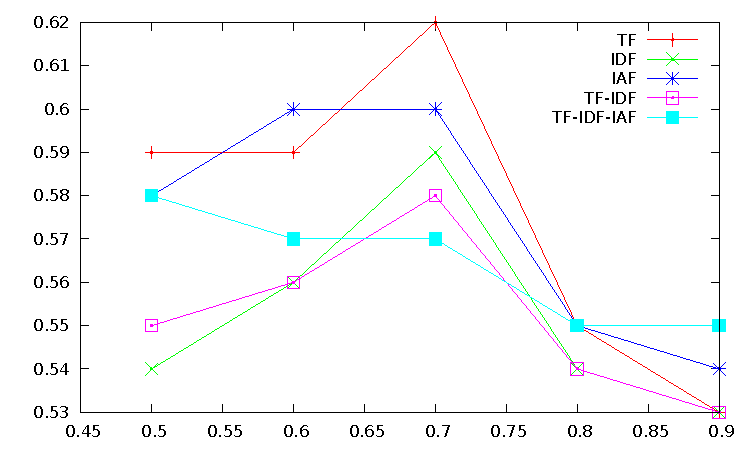
\includegraphics[width=140pt]{Figs/1-1.pdf} & 
%		\hspace{-6mm} 
		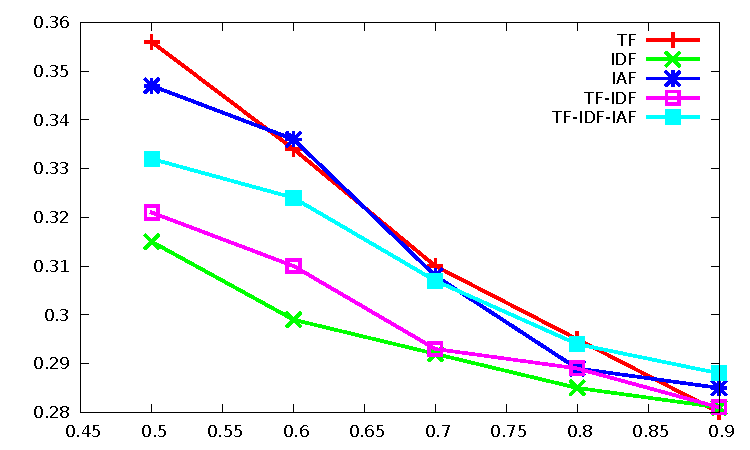
\includegraphics[width=140pt]{Figs/1-2.pdf} & 
%		\hspace{-10mm} 
		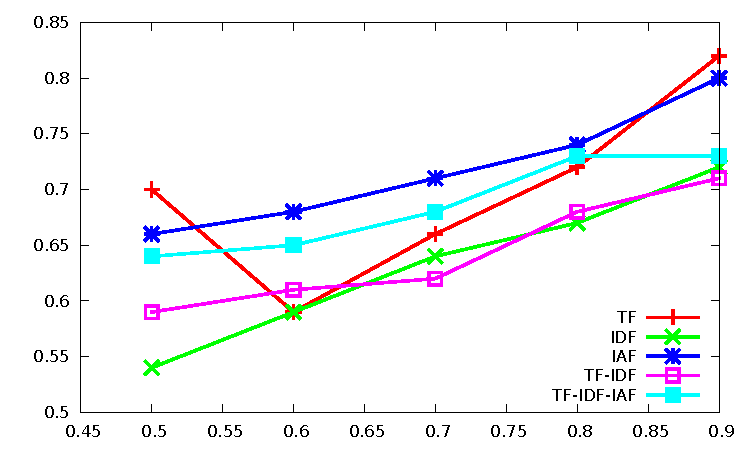
\includegraphics[width=140pt]{Figs/1-3.pdf} \\  
	
%		\vspace{4mm}
		{\footnotesize Purity (Generic)} & {\footnotesize NMI (Generic)} & 
		%\hspace{-3mm} 
		{\footnotesize PMI(Generic)}\\
	
%		\vspace{-2mm}
%		\hspace{-8mm} 
		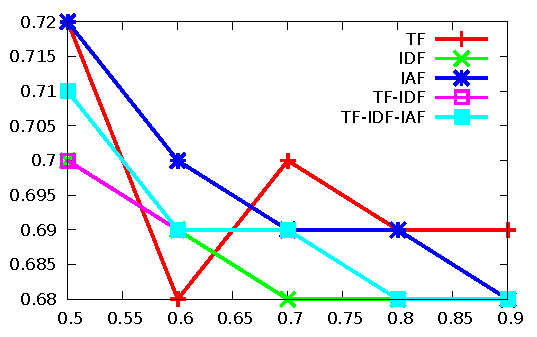
\includegraphics[width=140pt]{Figs/2-1.pdf} & 
%		\hspace{-6mm} 
		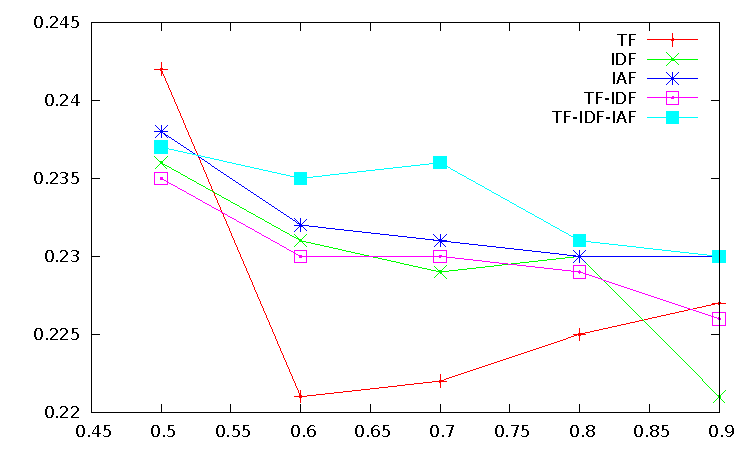
\includegraphics[width=140pt]{Figs/2-2.pdf} & 
%		\hspace{-10mm}
		 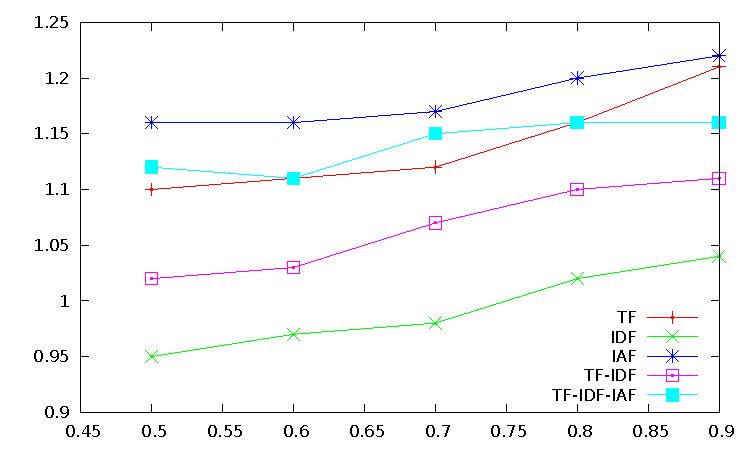
\includegraphics[width=140pt]{Figs/2-3.pdf} \\

		{\footnotesize Purity (Specific)} & {\footnotesize NMI (Specific)} & 
		%\hspace{-3mm} 
		{\footnotesize PMI(Specific)}\\


%		\vspace{-2mm}
%		\hspace{-1mm} 
		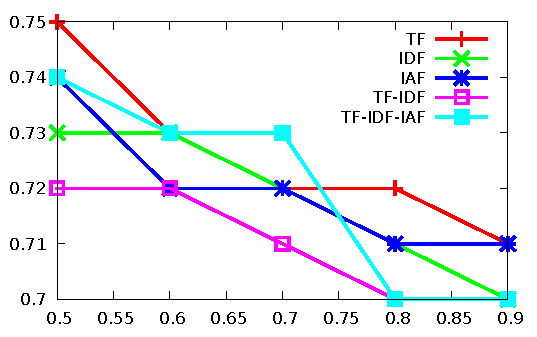
\includegraphics[width=140pt]{Figs/3-1.pdf} & 
%		\hspace{-1mm} 
		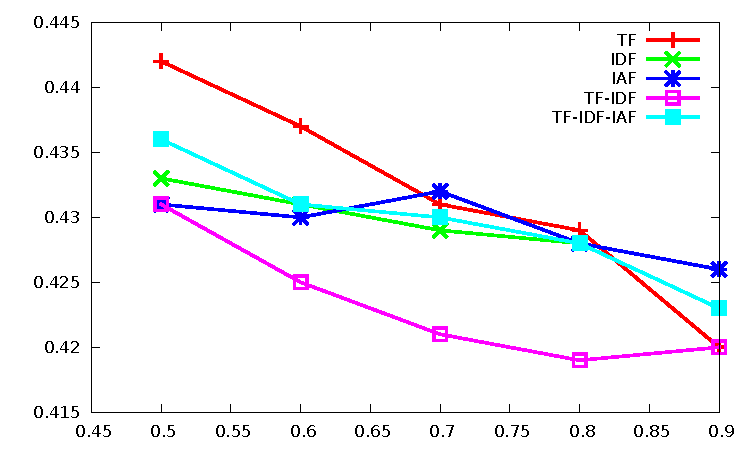
\includegraphics[width=140pt]{Figs/3-2.pdf} & 
		%\hspace{-1mm}
		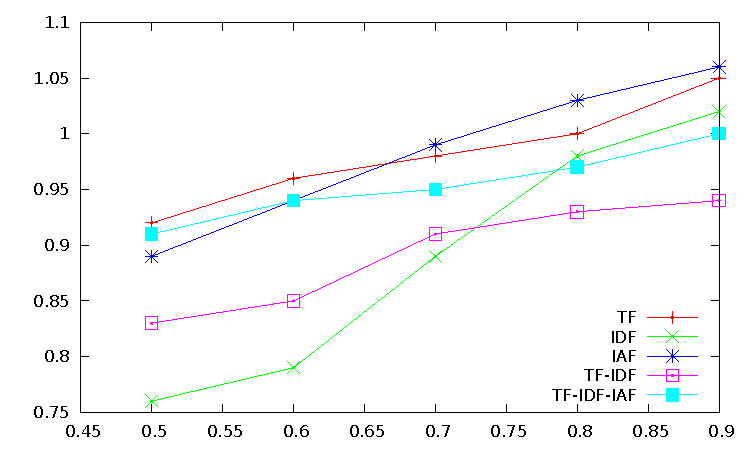
\includegraphics[width=140pt]{Figs/3-3.pdf} \\

		
%		\vspace{4mm}

		{\footnotesize Purity (Events)} & {\footnotesize NMI (Events)} & 
		%\hspace{-3mm} 
		{\footnotesize PMI(Events)}\\

	
	\end{tabular}
}
\end{center}
\vspace{-4mm}
\caption{\footnotesize Comparison of Purity, NMI and PMI scores for different similarity metrics for Hashtag Assignment.} \label{fig-1}
\end{figure*}
%%%%%%%%%%%%%%%%%%%%%%%%%%%%%%%%%%%%%%%%%%%%%%%%%%%%%%%%%%%%%%%%%%%%%%%%%%




\section{Overall Comparison}
The goal of this work was to get better topics which have better coherence, interpretability and usability without modifying the basic machinery of standard LDA. The default way of using tweets to train LDA was to treat each tweet as a single document (referred in this work as the Unpooled scheme). Simple hashtag based pooling outperformed unpooled scheme and other pooling schemes while hashtag assignment further improved results. Table~\ref{tbl-10} provides an overall comparison of the different schemes: Unpooled vs simple hashtag vs hashtag assignment on the three datasets.

\begin{table}[!h]
%\setcounter{table}{13}
\centering
\resizebox{14cm}{!} 
{
	\begin{tabular}{|l|ccc|ccc|ccc|}
	\hline
	Pooling Scheme  & \multicolumn {3}{c}{Purity} & \multicolumn {3}{c}{NMI Scores} & \multicolumn {3}{c|}{PMI Scores}\\
	\hline
	 & Generic & Specific & Events &  Generic & Specific & Events &  Generic & Specific & Events\\
	\hline
	Unpooled & 0.49 & 0.64 & 0.69 & 0.29 & 0.22 & 0.39 & -1.27 & 0.47 & 0.47 \\
	\hline
	Basic Hashtagwise & 0.53 & 0.68 & 0.71 & 0.28 & 0.23 & 0.42 & 0.78 & \textbf{1.43} & \textbf{1.07} \\
	\hline
	Tag-Assignment & \textbf{0.62} & \textbf{0.72} & \textbf{0.75} & \textbf{0.36} & \textbf{0.24} & \textbf{0.44} & \textbf{0.82} & 1.21 & 1.05 \\
	\hline
	\end{tabular}
}
\caption{Overall comparison of improvement}\label{tbl-10}
\end{table}


\section{Observations}
The work described in this paper presents a way of aggregating tweets in order to improve performance of topic models in terms of quality of topics obtained  measures by the ability to reconstruct clusters and topic coherence. The initial results presented in Table~\ref{tbl-4}, ~\ref{tbl-5} and ~\ref{tbl-6} suggest that hashtag based pooling outperforms all other pooling strategies including the default way of training topic models on Twitter data(unpooled).
\\\\
Since a major portion of Twitter data does not contains hashtags we looked at ways of assigning hashtags to tweets. Insights from Hashtag Assignment results (Table~\ref{tbl-9}) suggest that when the main aim is to use the topics obtained to extract different events mentioned in the Twitter data one should use hashtag assignment with a relaxed threshold(~0.5). The high values of Purity scores and NMI values for low threshold support this claim.
\\\\
When the goal is to obtain interesting topics with topic words pertaining to the same common theme (coherent topic words), hashtag assignment with strict constraints(threshold ~ 0.9) works well. The PMI scores in Table~\ref{tbl-9} highlight that topic coherence increases as we move down the column. Thus the threshold of 0.9 gives most coherent topics.
\\\\
Overall, results shown in Table~\ref{tbl-10} compare unpooled scheme with simple hashtag pooling and hashtag assignment schemes. The best Purity and NMI scores are obtained by hashtag assignment while even the simple hashtag based pooling scheme working much better than the default way of unpooled tweets. When the dataset in consideration consists of generic terms simple hashtag pooling gives the best results in terms of topic coherence. On the other hand when we have tweets on specific named entities or events in general one might want to prefer hashtag assignment as it results in best PMI scores. 
\\


\section{Related Work}
Topic modelling is widely used in text mining communities with LDA
being the benchmark.  LDA has been extended in a variety of ways, and
in particular for social networks and social media, a number of
extensions to LDA have been proposed.  For example, \cite{newman11} proposed
two methods to regularize the learning of topic models aimed at short
text snippets. While the focus of this work was on blogs and search
result snippets, it would be interesting to see how well they work on
Twitter data. Also, the combination of the work proposed in this paper
with the tweet pooling schemes we describe before could produce
interesting results.


%There are other recent approaches for microblog retrieval, including estimating text quality of each tweet [ISTI-TREC2011], designing tweet informativeness and user/social features [Yandex-TREC2011] but these are not focused on improving LDA.

%For hashtag recommendataion, [MazziaUMich] uses naive bayes model, and \cite{zangerle2011recommending} _also_ uses tweet similarity as a criteria. Moreover, the fraction of tweets with hashtags is observed as ~30+% on a large corpus, higher than what was observed on the three datasets here.


%Among the social networks, several characteristics of the data available in microblogs make them appealing for applications which fall into three broad categories: event detection [3], trend identification [4], and social group identification [5]. The interested reader is directed to the work of Liao et al[9] which discusses the opportunities and challenges related to mining microblogs.

Our work is quite different from many pioneering studies on Twitter and topic modeling because we try to study how we could get better topics using tweets with minimalistic efforts. Prior work on topic modeling for tweets includes the work of \cite{ramage} which presents a scalable implementation of a partially supervised learning model (Labeled LDA) that maps the content of the Twitter feed into dimensions and characterize users and tweets using this model. \cite{wayne} empirically compare the content of Twitter with a traditional news medium, New York Times, using unsupervised topic modeling. \cite{hong} use the topic modeling approach for predicting popular Twitter messages and classifying Twitter users and corresponding messages into topical categories. 

The {T}witterRank system~\cite{Weng2010wsdm} and \cite{hong} uses author-based pooling to apply LDA to tweets. \cite{Zhao2011ecir} compared topic characteristics between twitter and traditional news media (NY Times). It proposes to use one topic per tweet (in a manner similar to PLSA), and argues (with some evidence) that this is better than no pooling, or author-topic model. \cite{kireyev2009} used term weighting to tackle term sparseness in LDA, the weights are derived from LSA vector length. \cite{Naveed2011cikm} used LDA for tweet retrieval. In addition, they used retweet as an indicator of "interestingness" to improve retrieval quality.

Our work is different from these in the sense that we provide a simple yet effective way which greatly improves the quality of topics obtained without making any major complicated modifications to standard LDA. The detailed experiments on a variety of datasets highlight which scheme works well for which kind of dataset and for which task.
\\
%Evaluating topic models has continued to be an active research topic with the aim of automatically evaluating topic models. Newman et l [10] introduce the task of topic coherence evaluation, whereby a set of words, as generated by a topic model, is rated for coherence or interpretability. Wallach [11] present evaluation methods based on the probability of held-out documents given a trained model.

\section{Conclusion}
In this paper we have proposed different tweet pooling schemes which produce topics which are representative of the events mentioned in the data and are coherent. With this work we aim to support% provide pointers to the correct direction of 
developing topic models for short text and microblogs. %We hope that the observations and results discussed in this paper will engender novel research on topic models for microblogs.

The Hashtag-based pooling scheme and tag assignment proposed works better than all other schemes across almost all datasets and metrics. It is encouraging that our simple algorithms produce good results across a broad spectrum of domains.
%\section*{Acknowledgments}
%NICTA is funded by the Australian Government as represented by the Department of Broadband, Communications and the Digital Economy and the Australian Research Council through the ICT Centre of Excellence program.

%'apalike-fr' style below applies smallcaps style on author names
%in order to apply 'apalike-fr' the babel package must be given [frenchb] option instead of [english]
% \usepackage[frenchb]{babel} also causes title "References" to render with French accents like "R\'ef\'erences"
%\bibliographystyle{apalike-fr}

%'apa' style does not apply "smallcaps style" on author names and goes with the [english] option in the babel package

%\bibliography{colingbiblio}
%\bibliographystyle{apa}




%\bibliography{sve}
%\bibliographystyle{aaai}


\bibliographystyle{apa}
\bibliography{colingbiblio}
% \nocite{*}
%\bibliographystyle{coling2012

%\nocite{TALN2007,LaigneletRioult09,LanglaisPatry07,au1972,cks1981,mb2012}

%%================================================================
\end{document}


Latent Dirichlet allocation (LDA) \cite{blei03} is a generative model for text. In LDA, each document may be viewed as a mixture of various topics. We use the following notations for describing the LDA model:\\
\hspace{2cm} M : number of documents\\
\hspace{2cm} N : number of words in a document\\
\hspace{2cm} $\alpha$ : parameter of the Dirichlet prior on the per-document topic   distributions\\
\hspace{2cm} $\beta$ : the parameter of the Dirichlet prior on the per-topic word distribution\\
\hspace{2cm} $\theta_i$ : the topic distribution for document i,\\
\hspace{2cm} $\phi_k$ is the word distribution for topic k,\\
\hspace{2cm} $z_{ik}$ is the topic for the jth word in document i, and\\
\hspace{2cm} $w_{ij}$ is the specific word.
 
The $w_{ij}$ are the only observable variables, and the other variables are latent variables. If K be the number of topics considered in the model, $\phi$ is a $K*V$ (V is the dimension of the vocabulary) matrix each row of which denotes the word distribution of a topic.

The generative process behind is that documents are represented as random mixtures over latent topics, where each topic is characterized by a distribution over words. LDA assumes the following generative process for each document i in a corpus D :

\begin{compactenum}
\item Choose $\phi_i \sim Dir(\alpha)$, where i $\in$ {1,...,M} and Dir($\alpha$) is the Dirichlet distribution for parameter $\alpha$
\item Chose $\phi_k \sim Dir(\beta)$, where k $\in {1,...,K}$
\item For each of the words $w_{ij}$, where j $\in {1,...,N_i}$
	\begin{compactenum}
		\item Chose a topic $z_{i,j} \sim Multinomial(\theta)$
		\item Chose a word $w_{i,j} \sim Multinomial(\phi_{z_{i,j}})$
	\end{compactenum}
\end{compactenum}


Learning the various distributions (the set of topics, their associated word probabilities, the topic of each word, and the particular topic mixture of each document) is a problem of Bayesian inference. The original paper used a variational Bayes approximation of the posterior distribution; alternative inference techniques use Gibbs sampling and expectation propagation.







%In this model, a “topic” t is a discrete distribution over words with probability vector $\phi_{t}$. Dirichlet priors, with concentration parameter $\beta$ and base measure $n$, are placed over the topics $\Phi = \lbrace \phi_{1}, ... , \phi_{T} \rbrace $ :

%\begin{center}
%$P\left( \Phi \right)  = \Pi_{t}  Dir\left(  \phi_{t} ; \beta n  \right) $
%\end{center}

%Each document, indexed by d, is assumed to have its own distribution over topics given by probabilities $\theta_{d}$. The priors over $\Theta = \lbrace  \theta_{1}, ... , \theta_{d}  \rbrace$ are also Dirichlet, with concentration parameter $\alpha$ and base measure $m$:

%\begin{center}
%$P\left( \Theta \right)  = \Pi_{d}  Dir\left(  \theta_{d} ; \alpha m  \right) $
%\end{center}

%The tokens in a document $w^{d} = \lbrace w^{d}_{n} \rbrace^{N_{d}}_{n=1} $ (where $N_d$ is the number of tokens in the document d)are associated with topic assignments $z^{d} = \lbrace z^{d}_{n} \rbrace^{N_{d}}_{n=1} $, drawn i.i.d. from the document-specific topic distribution:
%\begin{center}
%$P\left( z_{d} | \theta_{d}  \right) = \Pi_{n} \theta_{ z^{\left( d\right) }_{n} %| d}$.
%\end{center}
%The tokens are drawn from the topics’ distributions:
%\begin{center}
%$P\left( w_{d} | z_{d}, \Phi  \right) = \Pi_{n} \phi_{ w^{\left( d\right) }_{n} | z^{\left( d\right) }_{n}}$.
%\end{center}

%A data set of documents $W = \lbrace w^(1) , w^(2) , ..., w^(D) \rbrace $ is observed, while the underlying corresponding topic assignments $Z = \lbrace z^(1) , z^(2) , ..., z^(D) \rbrace $ are unobserved. 
%\\

